\documentclass[11pt]{article}
\usepackage[a4paper,margin=23mm]{geometry}
\usepackage[T1]{fontenc}
\usepackage{lmodern,amsmath,amssymb,amsthm,mathtools,microtype,enumitem,tikz}
\usepackage[colorlinks=true,linkcolor=blue,urlcolor=blue]{hyperref}
\hypersetup{pdftitle={zeta(3) is irrational: the maximum-principle proof, simplified},pdfauthor={Mathathon peer-review digest}}
\newcommand{\Z}{\mathbb Z}
\newcommand{\T}{\mathcal T}
\DeclareMathOperator{\lcm}{lcm}
\newcommand{\q}[1]{\medskip\noindent\textbf{#1}}
\setlist{itemsep=1pt,topsep=3pt}
\title{$\zeta(3)$ is irrational: the maximum-principle proof, simplified}
\author{Mathathon peer-review digest (Claude)}
\date{15 November 2026 \quad(draft 3, after independent reading)}
\begin{document}
\maketitle

\noindent\textbf{The destination.} We construct numbers
\[
I_n=2\bigl(a_n\zeta(3)-b_n\bigr),\qquad a_n\in\Z,\qquad D_n^3b_n\in\Z,\qquad D_n=\lcm(1,\dots,n)\quad(D_0=1).
\]
If $\zeta(3)$ were a fraction $P/Q$, then $\frac Q2D_n^3I_n$ would be an integer. So the whole point
is to show that $I_n$ is \emph{not zero} and is \emph{small compared with $D_n^{-3}$}, which is about
$20^{-n}$. The sum that defines $I_n$ gives much less: only that $I_n\to0$, about as fast as $1/n$,
and nothing about its sign. That alone proves nothing; the error $\zeta(3)-\sum_{k\le n}k^{-3}$ of the
partial sums also tends to zero, with the same denominators. A difference equation, read as a law
for currents in a chain, turns the weak fact into the strong one: $0<I_n\le2\zeta(3)\,33^{-n}$. Then
$D_n^3\ge33^n/P$ for every $n$. But an identity for $N!$ caps the growth rate of $D_n$ at $e$, and
$e^3=20.1<33$.

\smallskip\noindent Each section has one idea. \textbf{1:} poles for the arithmetic, zeros for the
size. \textbf{2:} one telescope turns the sum into a chain with a current law. \textbf{3:} a
sequence that tends to zero and cannot have a peak must fall all the way. \textbf{4:} count prime
powers in $N!$.

\section{The linear forms}

\q{The numbers.} Poles at $0,-1,\dots,-n$ produce shifted zeta sums with controlled denominators.
Zeros at $1,\dots,n$ remove the first $n$ terms. So let
\[
r_n(t)=\frac{(1-t)(2-t)\cdots(n-t)}{t\,(t+1)\cdots(t+n)},\qquad \T(f)=-\sum_{t\ge1}f'(t),\qquad
I_n=\T(r_n^2).
\]
The square makes the zeros survive the differentiation; the derivative produces the cubic poles.
Here $r_0=1/t$, so $I_0=\sum2t^{-3}=2\zeta(3)>0$.

\q{Arithmetic.} Write $e_k=\frac1{t+k}$ and $H^{(s)}_k=\sum_{l\le k}l^{-s}$. Then
$\T(e_k^2)=2\bigl(\zeta(3)-H^{(3)}_k\bigr)$ and $\T(e_k)=\zeta(2)-H^{(2)}_k$. Partial fractions give
$r_n=\sum_{k=0}^nc_ke_k$ with
\[
c_k=\Bigl[(t+k)\,r_n\Bigr]_{t=-k}=(-1)^k\frac{(n+k)!}{k!\,k!\,(n-k)!}\in\Z
\]
(a multinomial coefficient). Since $e_ke_j=\frac{e_k-e_j}{j-k}$ for $k\ne j$, the constant $\zeta(2)$
cancels in every mixed term:
\[
I_n=\sum_kc_k^2\,\T(e_k^2)+2\sum_{k<j}c_kc_j\,\frac{\T(e_k)-\T(e_j)}{j-k}
=2\Bigl(\sum_kc_k^2\Bigr)\zeta(3)-2\Bigl(\sum_kc_k^2H^{(3)}_k-\sum_{k<j}c_kc_j\frac{H^{(2)}_j-H^{(2)}_k}{j-k}\Bigr).
\]
So $I_n=2(a_n\zeta(3)-b_n)$ with $a_n=\sum c_k^2\in\Z$, and $D_n^3b_n\in\Z$: $D_n^3$ clears
$H^{(3)}_k$, and $D_n\cdot D_n^2$ clears $\frac1{j-k}\,H^{(2)}$.

\q{The only estimate we take from the sum.} Write $r_n=\frac1t\,\varphi_1\cdots\varphi_n$ with
$\varphi_j=\frac{j-t}{j+t}$. For $t>0$ we have $|\varphi_j|<1$ and
$|\varphi_j'|=\frac{2j}{(j+t)^2}\le\frac1{2t}$, because $(j+t)^2\ge4jt$. So $|r_n|\le\frac1t$. By the
product rule, $r_n'$ is a sum of $n+1$ terms, in each of which one factor of
$\frac1t\,\varphi_1\cdots\varphi_n$ is differentiated; so
$|r_n'|\le\frac1{t^2}+n\cdot\frac1t\cdot\frac1{2t}$, and $|(r_n^2)'|=2\,|r_n|\,|r_n'|\le\frac{n+2}{t^3}$. As
$(r_n^2)'$ vanishes at $t=1,\dots,n$,
\begin{equation}\label{bdd}
|I_n|\le(n+2)\sum_{t>n}\frac1{t^3}<(n+2)\sum_{t>n}\frac1{(t-1)\,t\,(t+1)}=\frac{n+2}{2n(n+1)}\qquad(n\ge1).
\end{equation}
(The last sum telescopes: $\frac1{(t-1)t(t+1)}=\frac12\bigl[\frac1{(t-1)t}-\frac1{t(t+1)}\bigr]$.) In
particular $I_n\to0$. But this is all: the bound decays only like $\frac1{2n}$, the terms of the sum
are not of one sign, and we control neither their cancellation nor the sign of the total. Sections
2 and 3 supply both.

\section{The recurrence: Ohm and Kirchhoff}

\q{The only tool.} Write $\Delta g(t)=g(t+1)-g(t)$. Let $g$ be a rational function with no pole at
$1,2,3,\dots$ and a zero of order at least two at $t=1$ (so $g'(1)=0$), and suppose that
$g'(t)\to\kappa$ as $t\to\infty$. Since $(\Delta g)'(t)=g'(t+1)-g'(t)$, the sum that defines
$\T(\Delta g)$ telescopes:
\begin{equation}\label{tel}
\T(\Delta g)=\lim_{N\to\infty}\bigl(g'(1)-g'(N+1)\bigr)=-\kappa .
\end{equation}
(Every sum $\T(f)$ below converges absolutely: $f$ is always a rational function with no pole at
$1,2,3,\dots$ and a finite limit at infinity, so $f'(t)=O(t^{-2})$.)

\q{Step 1: the drop lives on the link.} Picture $0,1,2,\dots$ as the nodes of a chain, with $I_n$
at node $n$. Neighbouring functions differ by one factor, $r_n=\frac{n-t}{n+t}\,r_{n-1}$, so both
are multiples of a function that belongs to the link between them:
\[
r_{n-1}=(n+t)\,v_n,\qquad r_n=(n-t)\,v_n,\qquad v_n=\frac{(1-t)\cdots(n-1-t)}{t\,(t+1)\cdots(t+n)}\qquad(n\ge1).
\]
\begin{center}
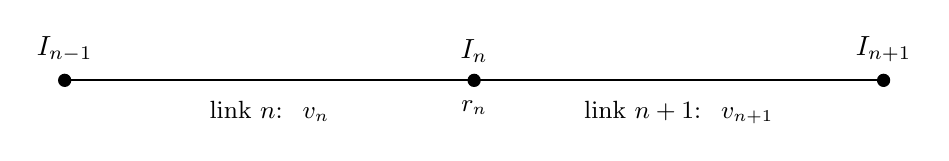
\begin{tikzpicture}[x=2.6cm,y=1cm]
\draw[thick] (0,0)--(4,0);
\foreach \x/\lab in {0/$I_{n-1}$,2/$I_n$,4/$I_{n+1}$} {\fill (\x,0) circle (2.4pt); \node[above=3pt] at (\x,0) {\lab};}
\node[below=4pt] at (1,0) {\small link $n$: \ $v_n$};
\node[below=4pt] at (3,0) {\small link $n+1$: \ $v_{n+1}$};
\node[below=4pt] at (2,0) {\small $r_n$};
\end{tikzpicture}
\end{center}
Since $(n+t)^2-(n-t)^2=4nt$, the drop across the link is
\begin{equation}\label{drop}
I_{n-1}-I_n=4n\,\T\bigl(t\,v_n^2\bigr).
\end{equation}

\q{Step 2: a function whose shift stays on the link.} To telescope we need a multiple of $v_n$ whose
shift is again a multiple of $v_n$. Shifting $t$ by one moves every zero and pole one step to the
left. So give $v_n$ one more zero on the right and one pole fewer on the left:
\begin{align*}
s_n(t)&=(n^2-t^2)\,v_n(t)=\frac{(1-t)\cdots(n-t)}{t\,(t+1)\cdots(t+n-1)},\\
s_n(t+1)&=\frac{(-t)(1-t)\cdots(n-1-t)}{(t+1)\cdots(t+n)}=-t^2\,v_n(t).
\end{align*}

\q{Step 3: the link identity.} The drop \eqref{drop} carries a factor $t$, so put a factor $t$ on
$s_n^2$:
\begin{equation}\label{link}
\Delta\bigl[t\,s_n^2\bigr]=\bigl[(t+1)\,t^4-t\,(n^2-t^2)^2\bigr]v_n^2=t^3\,(t+2n^2)\,v_n^2-n^4\,t\,v_n^2 .
\end{equation}
The last term is $n^4$ times what stands under $\T$ in \eqref{drop}. So the natural quantity on a
link is the \emph{current}
\[
J_n=n^3\,(I_{n-1}-I_n)=4\,\T\bigl(n^4\,t\,v_n^2\bigr):
\]
Ohm's law, with conductance $n^3$.

\q{Step 4: the node identity.} The first term on the right of \eqref{link} is the price of the
telescope, and it is paid at the node. The two links at node $n$ share $r_n=(n-t)\,v_n=(n+1+t)\,v_{n+1}$,
so $s_n=(n+t)\,r_n$ and $s_{n+1}=(n+1-t)\,r_n$, and Step~2 gives
$t^2v_n(t)=-(t+n+1)\,r_n(t+1)$ and $t^2v_{n+1}(t)=(t-n)\,r_n(t+1)$. Both prices are therefore
multiples of the same function:
\begin{equation}\label{node}
t^3(t+2n^2)\,v_n^2-t^3\bigl(t+2(n+1)^2\bigr)\,v_{n+1}^2=\frac{W(t)}t\,r_n(t+1)^2=(2n+1)^3\,r_n(t+1)^2 ,
\end{equation}
where $W(t)=(t+2n^2)(t+n+1)^2-\bigl(t+2(n+1)^2\bigr)(t-n)^2$. For the last step: the terms $t^3$
cancel, so $W$ has degree at most two, and its values at the three distinct points $0$, $n$,
$-n-1$ determine it. At $t=0$ the two products are equal. At $t=n$ only the first survives, at
$t=-n-1$ only the second. So $W(0)=0$, $W(n)=n(2n+1)^3$, $W(-n-1)=-(n+1)(2n+1)^3$, and hence
$W(t)=(2n+1)^3\,t$.

\q{Step 5: Kirchhoff's law.} Apply $\T$ to \eqref{link}. The function $t\,s_n^2$ has a double zero
at $t=1$, and its derivative tends to $1$, because $s_n^2=1+O(1/t)$. So \eqref{tel} gives $-1$ on
the left, and
\[
4\,\T\bigl(t^3(t+2n^2)\,v_n^2\bigr)=J_n-4 .
\]
Every link pays the same toll $4$. Now apply $\T$ to \eqref{node}. On the right,
$\T\bigl(r_n(t+1)^2\bigr)=-\sum_{t\ge2}(r_n^2)'(t)=I_n$, because $(r_n^2)'(1)=0$ for $n\ge1$. On the
left the two tolls cancel:
\begin{equation}\label{K}
\boxed{\;J_n-J_{n+1}=4\,(2n+1)^3\,I_n\qquad(n\ge1).\;}
\end{equation}
The current entering node $n$ either continues or is lost. Written out, this is Ap\'ery's recurrence
$(n+1)^3(I_{n+1}-I_n)-n^3(I_n-I_{n-1})=4(2n+1)^3I_n$.

\q{Where the coefficients come from.} The conductance $n^3$ is $n^4/n$: $n^4$ is the constant term
of $(n^2-t^2)^2$, and $n$ comes from $(n+t)^2-(n-t)^2=4nt$. The loss $(2n+1)^3$ is read off at the two
points $t=n$ and $t=-n-1$ where one of the two products in $W$ vanishes: at $t=n$, one factor $2n+1$
comes from $t+2n^2=n(2n+1)$ and two from $(t+n+1)^2$, the square of the distance between the two
points.

\q{The same law seen from the middle of a link (not needed).} The final version of the exposition
by Codex reaches \eqref{K} through one more number on each link, $E_n=\T(r_nr_{n-1})$, using the
telescope of the products $s_ns_m$ without the factor $t$. There $I_{n-1}+I_n=6\,E_n$, and this $6$
explains the constants in the usual form $(2n+1)\bigl(17n(n+1)+5\bigr)$ of the middle coefficient:
$17=6\cdot3-1$ and $5=6\cdot1-1$.

\section{The maximum principle}

We now forget the sum. Let $(X_n)_{n\ge0}$ be any real sequence satisfying the recurrence for all
$n\ge1$, and put
\[
F_n=n^3\,(X_n-X_{n-1})\quad(n\ge1),\qquad \ell_n=4(2n+1)^3 .
\]
Then the recurrence is the pair of rules
\begin{equation}\label{rules}
\boxed{\;F_{n+1}=F_n+\ell_nX_n,\qquad X_{n+1}=X_n+\frac{F_{n+1}}{(n+1)^3}\qquad(n\ge1)\;}
\end{equation}
$X_n$ is a \emph{height} and $F_n$ its \emph{weighted slope}. A positive height increases the next
slope. A positive next slope increases the next height. If both are negative, the same feedback
acts downward. The recurrence is a feedback rule, not just a formula for the next term.

\q{No positive peak, no negative valley.} If $X_n>0$ and $F_n\ge0$, the first rule gives
$F_{n+1}>0$: a positive height that has not just gone down must go up at the next step. So for
$n\ge1$ it is impossible that $X_n>0$, $X_n\ge X_{n-1}$ and $X_n\ge X_{n+1}$. In the same way a
negative valley is impossible. Only the signs of the weights were used.
\begin{center}
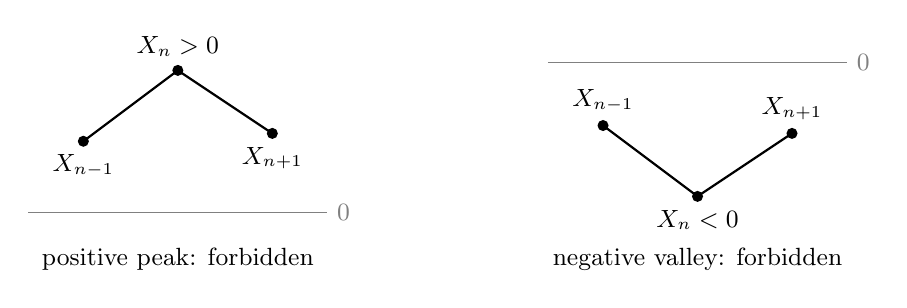
\begin{tikzpicture}[x=1cm,y=1cm]
\draw[gray] (-0.2,0)--(3.6,0) node[right] {\small $0$};
\draw[thick] (0.5,0.9)--(1.7,1.8)--(2.9,1.0);
\foreach \p in {(0.5,0.9),(1.7,1.8),(2.9,1.0)} \fill \p circle (2pt);
\node[below] at (0.5,0.85) {\small $X_{n-1}$}; \node[above] at (1.7,1.85) {\small $X_n>0$}; \node[below] at (2.9,0.95) {\small $X_{n+1}$};
\node[align=center] at (1.7,-0.6) {\small positive peak: forbidden};
\begin{scope}[xshift=6.6cm]
\draw[gray] (-0.2,1.9)--(3.6,1.9) node[right] {\small $0$};
\draw[thick] (0.5,1.1)--(1.7,0.2)--(2.9,1.0);
\foreach \p in {(0.5,1.1),(1.7,0.2),(2.9,1.0)} \fill \p circle (2pt);
\node[above] at (0.5,1.15) {\small $X_{n-1}$}; \node[below] at (1.7,0.15) {\small $X_n<0$}; \node[above] at (2.9,1.05) {\small $X_{n+1}$};
\node[align=center] at (1.7,-0.6) {\small negative valley: forbidden};
\end{scope}
\end{tikzpicture}
\end{center}

\q{A sequence that tends to zero attains every extreme other than $0$.} If one of its terms is
negative, say equal to $-\eta$, then only finitely many terms lie below $-\eta/2$, and the least of
these is the least term of the whole sequence. In the same way a positive term implies a largest
term. This is all we have to add, and Section~1 provides the two facts we need: $I_n\to0$ and
$I_0>0$.
\begin{enumerate}[label=(\alph*)]
\item \emph{No $I_n$ is negative.} Otherwise there is a least term, and it is negative. It is
$I_n$ for some $n\ge1$, because $I_0>0$. Then $I_n<0$, $I_n\le I_{n-1}$ and $I_n\le I_{n+1}$: a
negative valley.
\item \emph{No $I_n$ is zero.} If $I_n=0$ with $n\ge1$, the recurrence reads
$(n+1)^3I_{n+1}+n^3I_{n-1}=0$, and both neighbours are $\ge0$ by (a); so both vanish, and going back
we reach $I_0=0$.
\item \emph{The sequence decreases.} Suppose $I_n\ge I_{n-1}$ for some $n\ge1$. The numbers
$I_n,I_{n+1},\dots$ are positive by (a) and (b) and tend to zero, so one of them is the largest; say
$I_m$ with $m\ge n$. Then $I_m>0$, $I_m\ge I_{m+1}$, and $I_m\ge I_{m-1}$ (by the choice of $m$ if
$m>n$, by assumption if $m=n$): a positive peak at $m\ge1$.
\end{enumerate}
Therefore
\[
0<I_n<I_{n-1}\qquad(n\ge1).
\]
This is the maximum principle in its plainest form: what vanishes at infinity and cannot have a
peak must fall all the way.

\q{Why decrease becomes exponential decay.} Positivity and decrease say that the current
$J_n=-F_n=n^3(I_{n-1}-I_n)$ is positive. The first rule is \eqref{K} again:
\[
J_n=J_{n+1}+\ell_nI_n .
\]
Think of the height $I_n$ as a voltage. The link to its left has conductance $n^3$, so the current
through it is $n^3$ times the voltage drop. At node $n$ the current either continues to the right
or leaks to ground.
\begin{center}
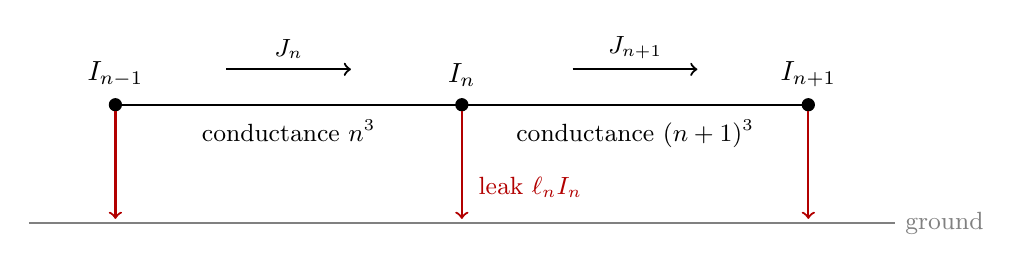
\begin{tikzpicture}[x=4.4cm,y=1cm]
\draw[thick] (0,0)--(2,0);
\foreach \x/\lab in {0/$I_{n-1}$,1/$I_n$,2/$I_{n+1}$} {\fill (\x,0) circle (2.4pt); \node[above=3pt] at (\x,0) {\lab};}
\draw[->,thick] (0.32,0.45)--(0.68,0.45) node[midway,above] {\small $J_n$};
\draw[->,thick] (1.32,0.45)--(1.68,0.45) node[midway,above] {\small $J_{n+1}$};
\node[below=2pt] at (0.5,0) {\small conductance $n^3$}; \node[below=2pt] at (1.5,0) {\small conductance $(n+1)^3$};
\foreach \x in {0,1,2} {\draw[->,thick,red!70!black] (\x,-0.08)--(\x,-1.45);}
\node[right,red!70!black] at (1.02,-1.05) {\small leak $\ell_nI_n$};
\draw[gray,thick] (-0.25,-1.5)--(2.25,-1.5) node[right] {\small ground};
\end{tikzpicture}
\end{center}
The incoming current exceeds the local loss, because the continuing current is positive:
\[
n^3(I_{n-1}-I_n)>\ell_nI_n,\qquad\text{that is,}\qquad
\frac{I_{n-1}}{I_n}>1+\frac{\ell_n}{n^3}=1+4\Bigl(2+\frac1n\Bigr)^3>33 .
\]
Therefore
\begin{equation}\label{decay}
\boxed{\;0<I_n\le2\zeta(3)\,33^{-n}\;}
\end{equation}
The $33$ has a meaning: one copy of $I_n$ remains, and the local loss requires more than $32$
further copies in the preceding voltage.

\q{What happens without the loss?} Then $J_n$ is constant and the drops are constant multiples of
$1/n^3$. The solution that tends to zero is a multiple of $\sum_{k>n}k^{-3}$, which decays only like
$n^{-2}$: the approximation of $\zeta(3)$ by its partial sums. The successful and the failed
approximation obey the same current law. What turns polynomial decay into exponential decay is
that the loss is more than $32$ times the conductance.

\q{What about the other solutions? (not needed).} In the plane of the pairs $(X_n,F_n)$ the two
quadrants where height and slope have the same sign are traps. If $X_n\ge0$ and $F_n\ge0$, not both
zero, the rules \eqref{rules} make both positive at the next step, and from then on
$X_{n+1}\ge\bigl(1+\ell_n/(n+1)^3\bigr)X_n>14X_n$, because $\frac{2n+1}{n+1}\ge\frac32$: the solution
explodes.
\begin{center}
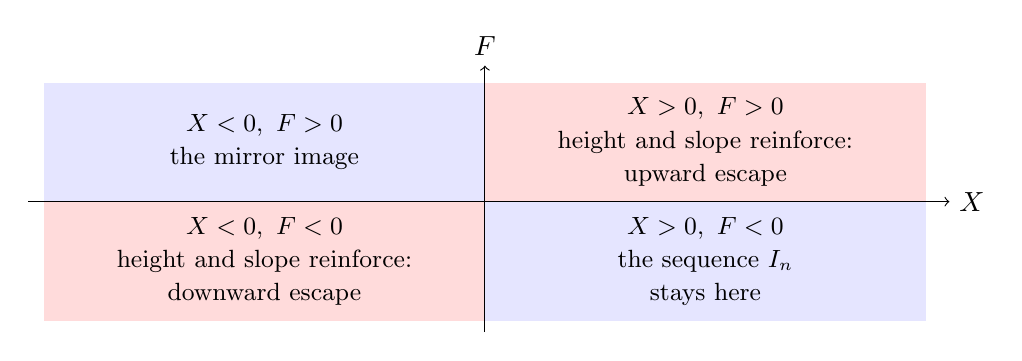
\begin{tikzpicture}[x=1cm,y=0.72cm]
\fill[red!14] (0,0) rectangle (5.6,2.1); \fill[red!14] (0,0) rectangle (-5.6,-2.1);
\fill[blue!10] (0,0) rectangle (5.6,-2.1); \fill[blue!10] (0,0) rectangle (-5.6,2.1);
\draw[->] (-5.8,0)--(5.9,0) node[right] {$X$}; \draw[->] (0,-2.3)--(0,2.4) node[above] {$F$};
\node[align=center] at (2.8,1.05) {\small $X>0,\ F>0$\\ \small height and slope reinforce:\\ \small upward escape};
\node[align=center] at (-2.8,-1.05) {\small $X<0,\ F<0$\\ \small height and slope reinforce:\\ \small downward escape};
\node[align=center] at (2.8,-1.05) {\small $X>0,\ F<0$\\ \small the sequence $I_n$\\ \small stays here};
\node[align=center] at (-2.8,1.05) {\small $X<0,\ F>0$\\ \small the mirror image};
\end{tikzpicture}
\end{center}
A solution with $X_0=0$ and $X_1\ne0$ starts in a trap, since $F_1=X_1$; so it is unbounded. Now
let $(X_n)$ be any bounded solution. Then $X_n-\frac{X_0}{I_0}I_n$ is a bounded solution that
vanishes at $n=0$; so it vanishes at $n=1$ too, and hence for all $n$. So every bounded solution is
a multiple of $(I_n)$: the solutions form a plane, and all of them except one line explode. That is
why so little information about the sum was enough.

\section{The denominator cost, and the contradiction}

\q{An identity.} $N!=\prod_{k=1}^ND_{\lfloor N/k\rfloor}$. Both sides are the product of $p$ over all
pairs $(k,q)$ with $k\ge1$, $q=p^a$ a prime power ($a\ge1$) and $kq\le N$: on the left because each $m\le N$ is the
product of $p$ over the prime powers $q$ dividing it (write $m=kq$), on the right because $D_M$ is
the product of $p$ over the prime powers $q\le M$.

\q{The growth rate of $D_n$ is at most $e$.} Suppose $D_m\ge c\,\lambda^m$ for all $m\ge1$, with
$c>0$ and $\lambda\ge1$. The identity has $N$ factors, each with an index $\lfloor N/k\rfloor\ge1$, so
$N!\ge c^N\lambda^{S}$ with $S=\sum_{k\le N}\lfloor N/k\rfloor$. Now
$S>N\bigl(\sum_{k\le N}\frac1k-1\bigr)>N(\log N-1)$, and $\lambda\ge1$; hence
\[
N^N\ge N!\ge c^N\lambda^{N(\log N-1)}\qquad\text{for every }N\ge1 .
\]
Take $N$-th roots and use $\lambda^{\log N}=N^{\log\lambda}$: this is $N\ge\frac c\lambda\,N^{\log\lambda}$.
If $\log\lambda>1$, it fails for large $N$. So $\log\lambda\le1$.

\q{The contradiction.} Suppose $\zeta(3)=P/Q$ with positive integers $P,Q$. Then
$\frac Q2D_n^3I_n=P\,D_n^3a_n-Q\,D_n^3b_n$ is an integer, and it is positive, so it is at least $1$. By
\eqref{decay},
\[
D_n^3\ge\frac2{Q\,I_n}\ge\frac{33^n}{Q\,\zeta(3)}=\frac{33^n}P\qquad\text{for every }n .
\]
So $D_n\ge P^{-1/3}\,(33^{1/3})^n$ for all $n$, and therefore $33^{1/3}\le e$. But $e^3=20.08\ldots<33$.
Hence $\zeta(3)$ is irrational.

\section*{Further intuition: the exact rate}

The bound $33^{-n}$ threw away the continuing current. Keep it. With $g_n=I_n/I_{n-1}\in(0,1)$,
dividing $J_n=J_{n+1}+\ell_nI_n$ by $n^3I_n$ gives
\[
\frac1{g_n}=1+4\Bigl(2+\frac1n\Bigr)^3+\Bigl(1+\frac1n\Bigr)^3(1-g_{n+1})=34-g_{n+1}+\delta_n,
\]
where $\delta_n=4\bigl[(2+\frac1n)^3-8\bigr]+\bigl[(1+\frac1n)^3-1\bigr](1-g_{n+1})$. The two brackets
are positive and at most $\frac{19}n$ and $\frac7n$, and $0<1-g_{n+1}<1$; so $0<\delta_n<\frac{83}n$.
The number $34$ is $1+32+1$: the present voltage, the limiting local loss, and the continuing
current. With the increasing function $f(x)=\frac1{34-x}$ this says $g_n=f(g_{n+1}-\delta_n)$.

\emph{The largest ratio reproduces itself.} Let $\sigma=\sup_ng_n\le1$. Then
$g_n<f(g_{n+1})\le f(\sigma)$ for every $n$, so $\sigma\le f(\sigma)$, that is,
$\sigma^2-34\sigma+1\ge0$. The roots are $\rho=17-12\sqrt2=0.0294$ and $1/\rho>1$, so
$\sigma\le\rho$, and
$0<I_n\le2\zeta(3)\,(17-12\sqrt2)^n$ for all $n$.

\emph{So does the smallest limit.} Let $L=\liminf g_n$ and $\varepsilon>0$. For all large $n$,
$g_{n+1}>L-\varepsilon$ and $\delta_n<\varepsilon$, hence $g_n>f(L-2\varepsilon)$. As $f$ is continuous, $L\ge f(L)$,
that is, $L^2-34L+1\le0$, that is, $L\ge\rho$. Together: $I_n/I_{n-1}\to17-12\sqrt2$.

\bigskip
\noindent\textbf{Status and sources.} Checked by AI agents only; no human has read it. An
independent AI reader went through draft~2 line by line and by computer (exact arithmetic for the
identities of Section~2 up to $n=14$, the recurrence on the linear forms up to $n=39$, the bounds of
Sections 1 and 3 up to $n=80$, the factorial identity up to $N=600$). It found no mathematical
error; its corrections are incorporated, among them the present form of Step~5. Who found what:
the link and node identities of Section~2, the bound \eqref{bdd} and its use in Section~3, and the
form of Section~4 are due to AI agents asked to simplify the exposition; the midpoint route and
the constants $6$ and $17$ are from the final version of the exposition by Codex, whose height,
slope and current language and pictures are kept here. The proof is a rearrangement of known
ideas: the series is that of W.~Zudilin's elementary proof (arXiv:math/0202159), and adding up the
pieces of Step~5 gives one quarter of the certificate used there; that Ap\'ery's linear forms are
the bounded solution of a recurrence with dominant middle coefficient is in A.~Mingarelli
(arXiv:math/0608577), and the constant $33$ in Mahboubi and Sibut-Pinote (arXiv:1912.06611).
\end{document}
